% Options for packages loaded elsewhere
\PassOptionsToPackage{unicode}{hyperref}
\PassOptionsToPackage{hyphens}{url}
\PassOptionsToPackage{dvipsnames,svgnames,x11names}{xcolor}
%
\documentclass[
  11pt,
  a4paper]{article}

\usepackage{amsmath,amssymb}
\usepackage{iftex}
\ifPDFTeX
  \usepackage[T1]{fontenc}
  \usepackage[utf8]{inputenc}
  \usepackage{textcomp} % provide euro and other symbols
\else % if luatex or xetex
  \usepackage{unicode-math}
  \defaultfontfeatures{Scale=MatchLowercase}
  \defaultfontfeatures[\rmfamily]{Ligatures=TeX,Scale=1}
\fi
\usepackage{lmodern}
\ifPDFTeX\else  
    % xetex/luatex font selection
\fi
% Use upquote if available, for straight quotes in verbatim environments
\IfFileExists{upquote.sty}{\usepackage{upquote}}{}
\IfFileExists{microtype.sty}{% use microtype if available
  \usepackage[]{microtype}
  \UseMicrotypeSet[protrusion]{basicmath} % disable protrusion for tt fonts
}{}
\makeatletter
\@ifundefined{KOMAClassName}{% if non-KOMA class
  \IfFileExists{parskip.sty}{%
    \usepackage{parskip}
  }{% else
    \setlength{\parindent}{0pt}
    \setlength{\parskip}{6pt plus 2pt minus 1pt}}
}{% if KOMA class
  \KOMAoptions{parskip=half}}
\makeatother
\usepackage{xcolor}
\usepackage[top=2.5cm,bottom=2.5cm,left=2.5cm,right=2.5cm]{geometry}
\setlength{\emergencystretch}{3em} % prevent overfull lines
\setcounter{secnumdepth}{5}
% Make \paragraph and \subparagraph free-standing
\makeatletter
\ifx\paragraph\undefined\else
  \let\oldparagraph\paragraph
  \renewcommand{\paragraph}{
    \@ifstar
      \xxxParagraphStar
      \xxxParagraphNoStar
  }
  \newcommand{\xxxParagraphStar}[1]{\oldparagraph*{#1}\mbox{}}
  \newcommand{\xxxParagraphNoStar}[1]{\oldparagraph{#1}\mbox{}}
\fi
\ifx\subparagraph\undefined\else
  \let\oldsubparagraph\subparagraph
  \renewcommand{\subparagraph}{
    \@ifstar
      \xxxSubParagraphStar
      \xxxSubParagraphNoStar
  }
  \newcommand{\xxxSubParagraphStar}[1]{\oldsubparagraph*{#1}\mbox{}}
  \newcommand{\xxxSubParagraphNoStar}[1]{\oldsubparagraph{#1}\mbox{}}
\fi
\makeatother


\providecommand{\tightlist}{%
  \setlength{\itemsep}{0pt}\setlength{\parskip}{0pt}}\usepackage{longtable,booktabs,array}
\usepackage{calc} % for calculating minipage widths
% Correct order of tables after \paragraph or \subparagraph
\usepackage{etoolbox}
\makeatletter
\patchcmd\longtable{\par}{\if@noskipsec\mbox{}\fi\par}{}{}
\makeatother
% Allow footnotes in longtable head/foot
\IfFileExists{footnotehyper.sty}{\usepackage{footnotehyper}}{\usepackage{footnote}}
\makesavenoteenv{longtable}
\usepackage{graphicx}
\makeatletter
\newsavebox\pandoc@box
\newcommand*\pandocbounded[1]{% scales image to fit in text height/width
  \sbox\pandoc@box{#1}%
  \Gscale@div\@tempa{\textheight}{\dimexpr\ht\pandoc@box+\dp\pandoc@box\relax}%
  \Gscale@div\@tempb{\linewidth}{\wd\pandoc@box}%
  \ifdim\@tempb\p@<\@tempa\p@\let\@tempa\@tempb\fi% select the smaller of both
  \ifdim\@tempa\p@<\p@\scalebox{\@tempa}{\usebox\pandoc@box}%
  \else\usebox{\pandoc@box}%
  \fi%
}
% Set default figure placement to htbp
\def\fps@figure{htbp}
\makeatother

\makeatletter
\@ifpackageloaded{caption}{}{\usepackage{caption}}
\AtBeginDocument{%
\ifdefined\contentsname
  \renewcommand*\contentsname{Table of contents}
\else
  \newcommand\contentsname{Table of contents}
\fi
\ifdefined\listfigurename
  \renewcommand*\listfigurename{List of Figures}
\else
  \newcommand\listfigurename{List of Figures}
\fi
\ifdefined\listtablename
  \renewcommand*\listtablename{List of Tables}
\else
  \newcommand\listtablename{List of Tables}
\fi
\ifdefined\figurename
  \renewcommand*\figurename{Figure}
\else
  \newcommand\figurename{Figure}
\fi
\ifdefined\tablename
  \renewcommand*\tablename{Table}
\else
  \newcommand\tablename{Table}
\fi
}
\@ifpackageloaded{float}{}{\usepackage{float}}
\floatstyle{ruled}
\@ifundefined{c@chapter}{\newfloat{codelisting}{h}{lop}}{\newfloat{codelisting}{h}{lop}[chapter]}
\floatname{codelisting}{Listing}
\newcommand*\listoflistings{\listof{codelisting}{List of Listings}}
\makeatother
\makeatletter
\makeatother
\makeatletter
\@ifpackageloaded{caption}{}{\usepackage{caption}}
\@ifpackageloaded{subcaption}{}{\usepackage{subcaption}}
\makeatother

\usepackage{bookmark}

\IfFileExists{xurl.sty}{\usepackage{xurl}}{} % add URL line breaks if available
\urlstyle{same} % disable monospaced font for URLs
\hypersetup{
  pdftitle={METIMMOX-1 Cost-Effectiveness Analysis Report},
  pdfauthor={Ben Geisler},
  colorlinks=true,
  linkcolor={blue},
  filecolor={Maroon},
  citecolor={Blue},
  urlcolor={Blue},
  pdfcreator={LaTeX via pandoc}}


\title{METIMMOX-1 Cost-Effectiveness Analysis Report}
\usepackage{etoolbox}
\makeatletter
\providecommand{\subtitle}[1]{% add subtitle to \maketitle
  \apptocmd{\@title}{\par {\large #1 \par}}{}{}
}
\makeatother
\subtitle{Biomarker-Guided Strategies for Selecting Immunotherapy
Candidates in Metastatic MSS/pMMR Colorectal Cancer}
\author{Ben Geisler}
\date{2025-10-07}

\begin{document}
\maketitle

\renewcommand*\contentsname{Table of contents}
{
\hypersetup{linkcolor=}
\setcounter{tocdepth}{3}
\tableofcontents
}

\section{Overview}\label{overview}

This cost-effectiveness analysis evaluates three biomarker-guided
strategies (CRP, TLR, and TMB/BRAF) for selecting metastatic
microsatellite stable (MSS)/proficient mismatch repair (pMMR) colorectal
cancer patients for immunotherapy versus the standard of care strategy
of chemotherapy alone.

This report contains:

\begin{itemize}
\tightlist
\item
  \textbf{Strategy Descriptions}: Overview of the four treatment
  strategies evaluated
\item
  \textbf{Base Case Analysis}: Cost-effectiveness results with
  incremental cost-effectiveness ratios (ICERs) and cost-effectiveness
  plane
\item
  \textbf{Deterministic Sensitivity Analysis}: Tornado diagrams showing
  parameter impact on each strategy
\item
  \textbf{Probabilistic Sensitivity Analysis}: Monte Carlo simulation
  results including scatterplot and cost-effectiveness acceptability
  curves
\end{itemize}

\section{Strategies Evaluated}\label{strategies-evaluated}

\begin{table}[H]
\caption{Treatment Strategies Evaluated in the Cost-Effectiveness Analysis}\tabularnewline

\centering\begingroup\fontsize{9}{11}\selectfont

\resizebox{\linewidth}{!}{
\begin{tabular}{>{\raggedright\arraybackslash}p{2.5cm}>{\raggedright\arraybackslash}p{8cm}>{\centering\arraybackslash}p{1.5cm}>{\centering\arraybackslash}p{1.5cm}}
\toprule
Strategy & Description & Biomarker Prevalence & Patients (n)\\
\midrule
Standard of Care & Standard of care - All patients receive only FLOX chemotherapy & 100.0\% & 36\\
CRP-guided Strategy & C-reactive protein with cut-off of <5 for biomarker-positive status. If CRP-positive: alternating two cycles each of FLOX (chemotherapy) and nivolumab (anti-PD1 immunotherapy); if CRP-negative: chemotherapy only & 33.8\% & 45\\
TLR-guided Strategy & Tumor Lesion Reduction with cut-off of >=10\% for biomarker-positive status. If TLR-positive: alternating two cycles each of FLOX (chemotherapy) and nivolumab (anti-PD1 immunotherapy); if TLR-negative: chemotherapy only & 64.7\% & 26\\
TMB/BRAF-guided Strategy & Combined biomarker: either Tumor Mutation Burden >= 9 or BRAF V600 mutation positive (both from next-generation sequencing). If TMB/BRAF-positive: alternating two cycles each of FLOX (chemotherapy) and nivolumab (anti-PD1 immunotherapy); if TMB/BRAF-negative: chemotherapy only & 44.9\% & 34\\
\bottomrule
\end{tabular}}
\endgroup{}
\end{table}

\newpage

\section{Base Case Analysis}\label{base-case-analysis}

\begin{longtable}[]{@{}lrrrllr@{}}
\caption{Base Case Cost-Effectiveness Results with ICERs}\tabularnewline
\toprule\noalign{}
Strategy & Cost & Effect & Inc\_Cost & Inc\_Effect & ICER & Status \\
\midrule\noalign{}
\endfirsthead
\toprule\noalign{}
Strategy & Cost & Effect & Inc\_Cost & Inc\_Effect & ICER & Status \\
\midrule\noalign{}
\endhead
\bottomrule\noalign{}
\endlastfoot
control & \$21,827 & 1.892 & NA & NA & NA & ND \\
crp & \$56,299 & 2.014 & 34471.96 & 0.121884 & \$282,826 & ND \\
tmb\_braf & \$68,664 & 1.944 & NA & NA & NA & D \\
tlr & \$77,574 & 1.359 & NA & NA & NA & D \\
\end{longtable}

\begin{figure}[H]

{\centering \pandocbounded{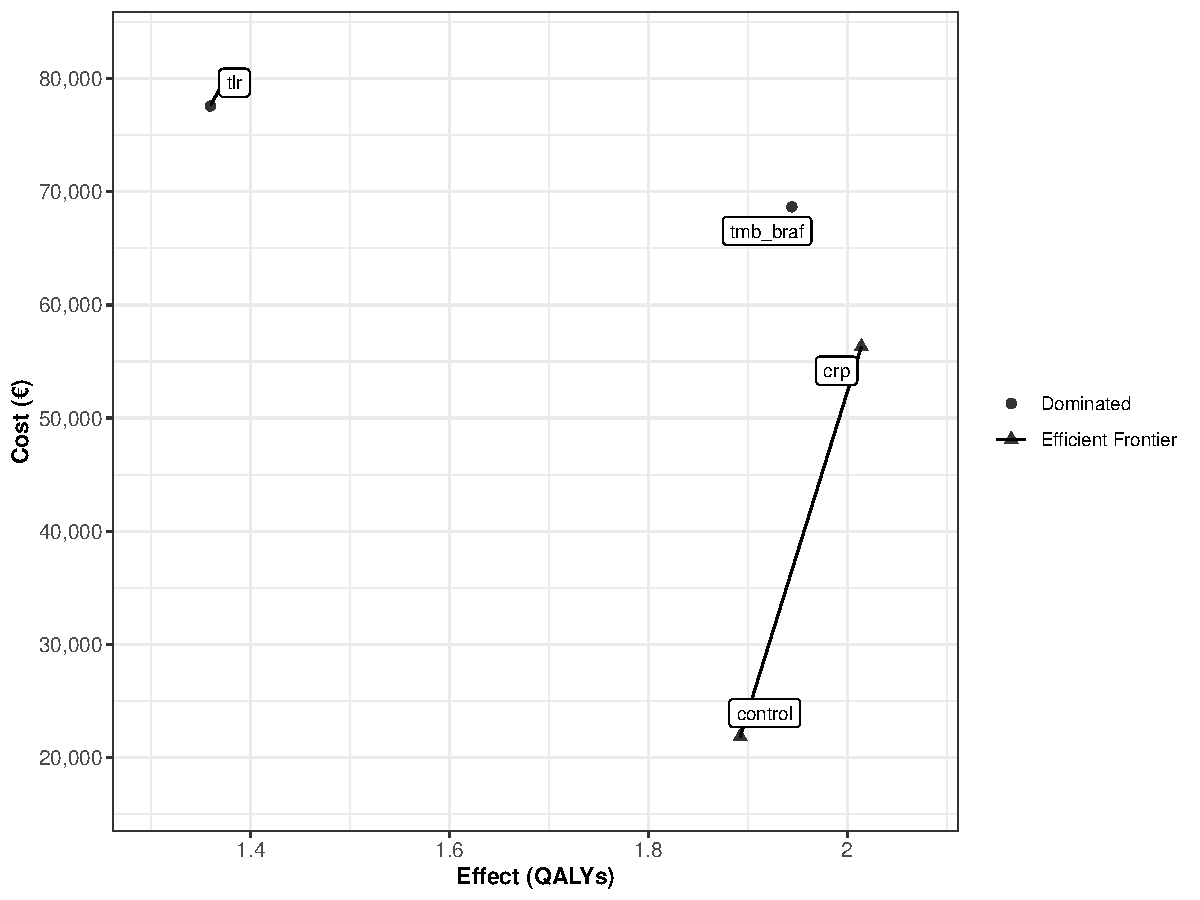
\includegraphics[keepaspectratio]{CEA_files/figure-pdf/cost-effectiveness-plane-1.pdf}}

}

\caption{Cost-Effectiveness Plane with Efficiency Frontier}

\end{figure}%

\section{Deterministic Sensitivity
Analysis}\label{deterministic-sensitivity-analysis}

\begin{figure}[H]

{\centering \pandocbounded{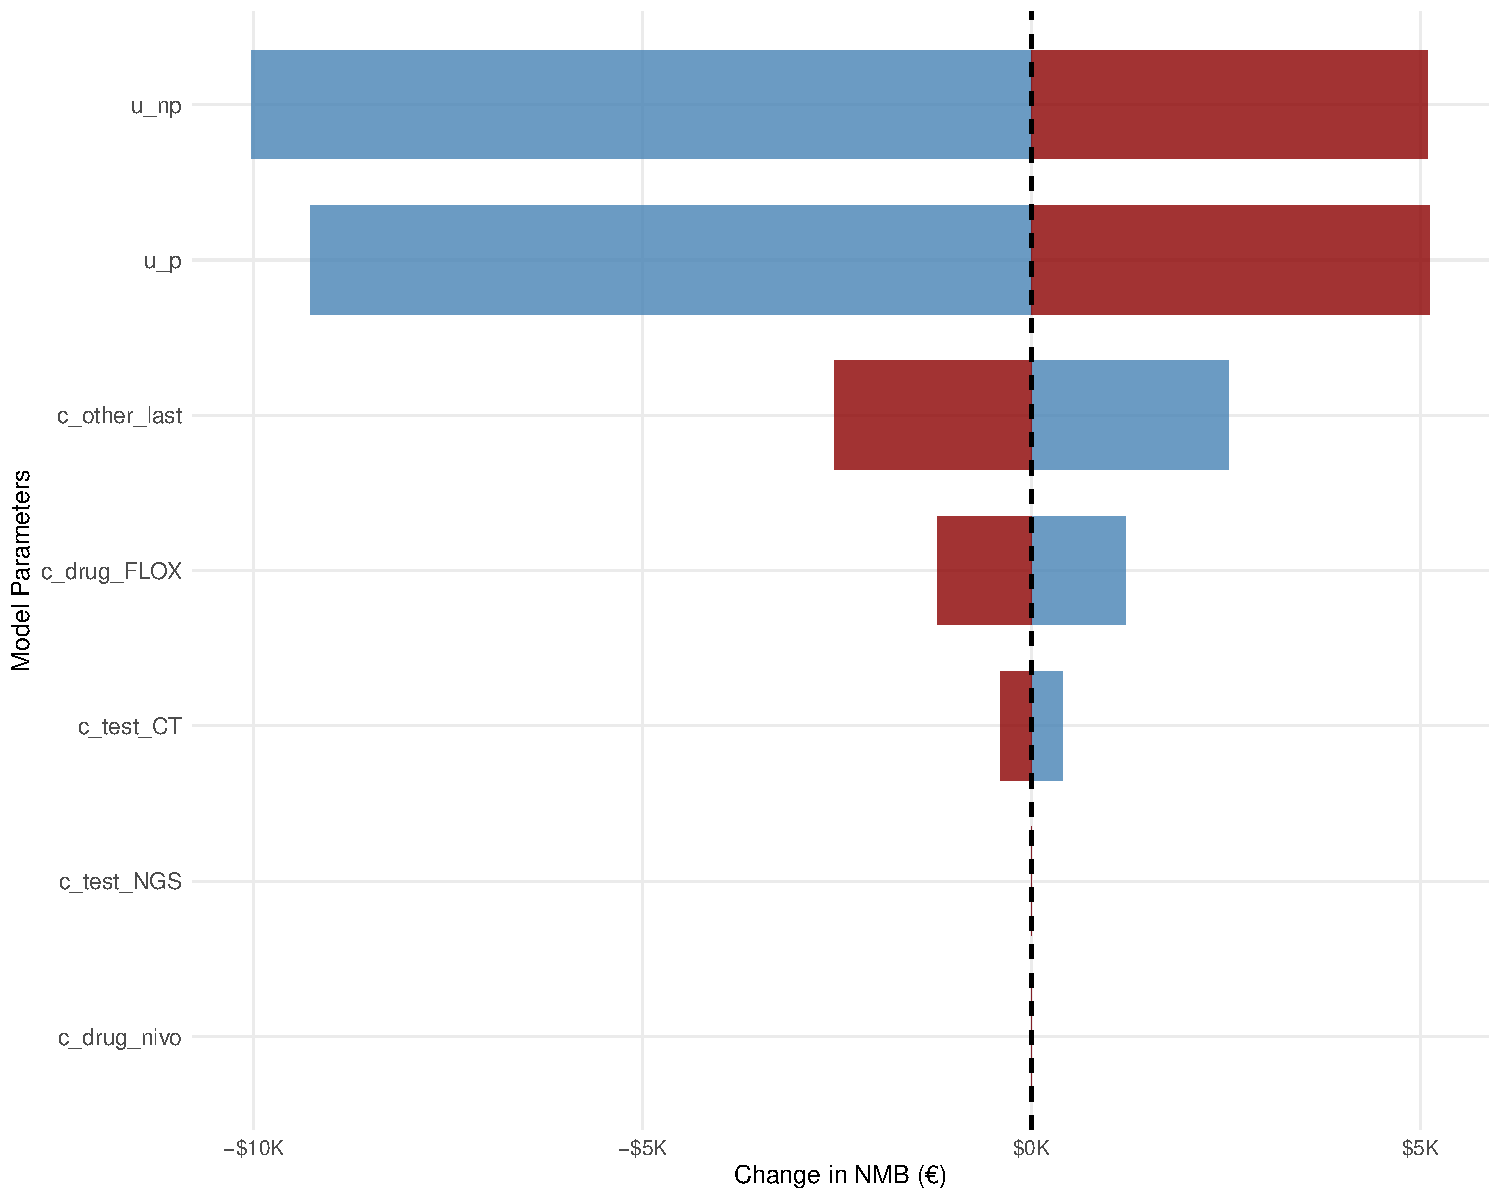
\includegraphics[keepaspectratio]{CEA_files/figure-pdf/tornado-control-1.pdf}}

}

\caption{Tornado Diagram - Standard of Care One-Way Sensitivity
Analysis}

\end{figure}%

\begin{figure}[H]

{\centering \pandocbounded{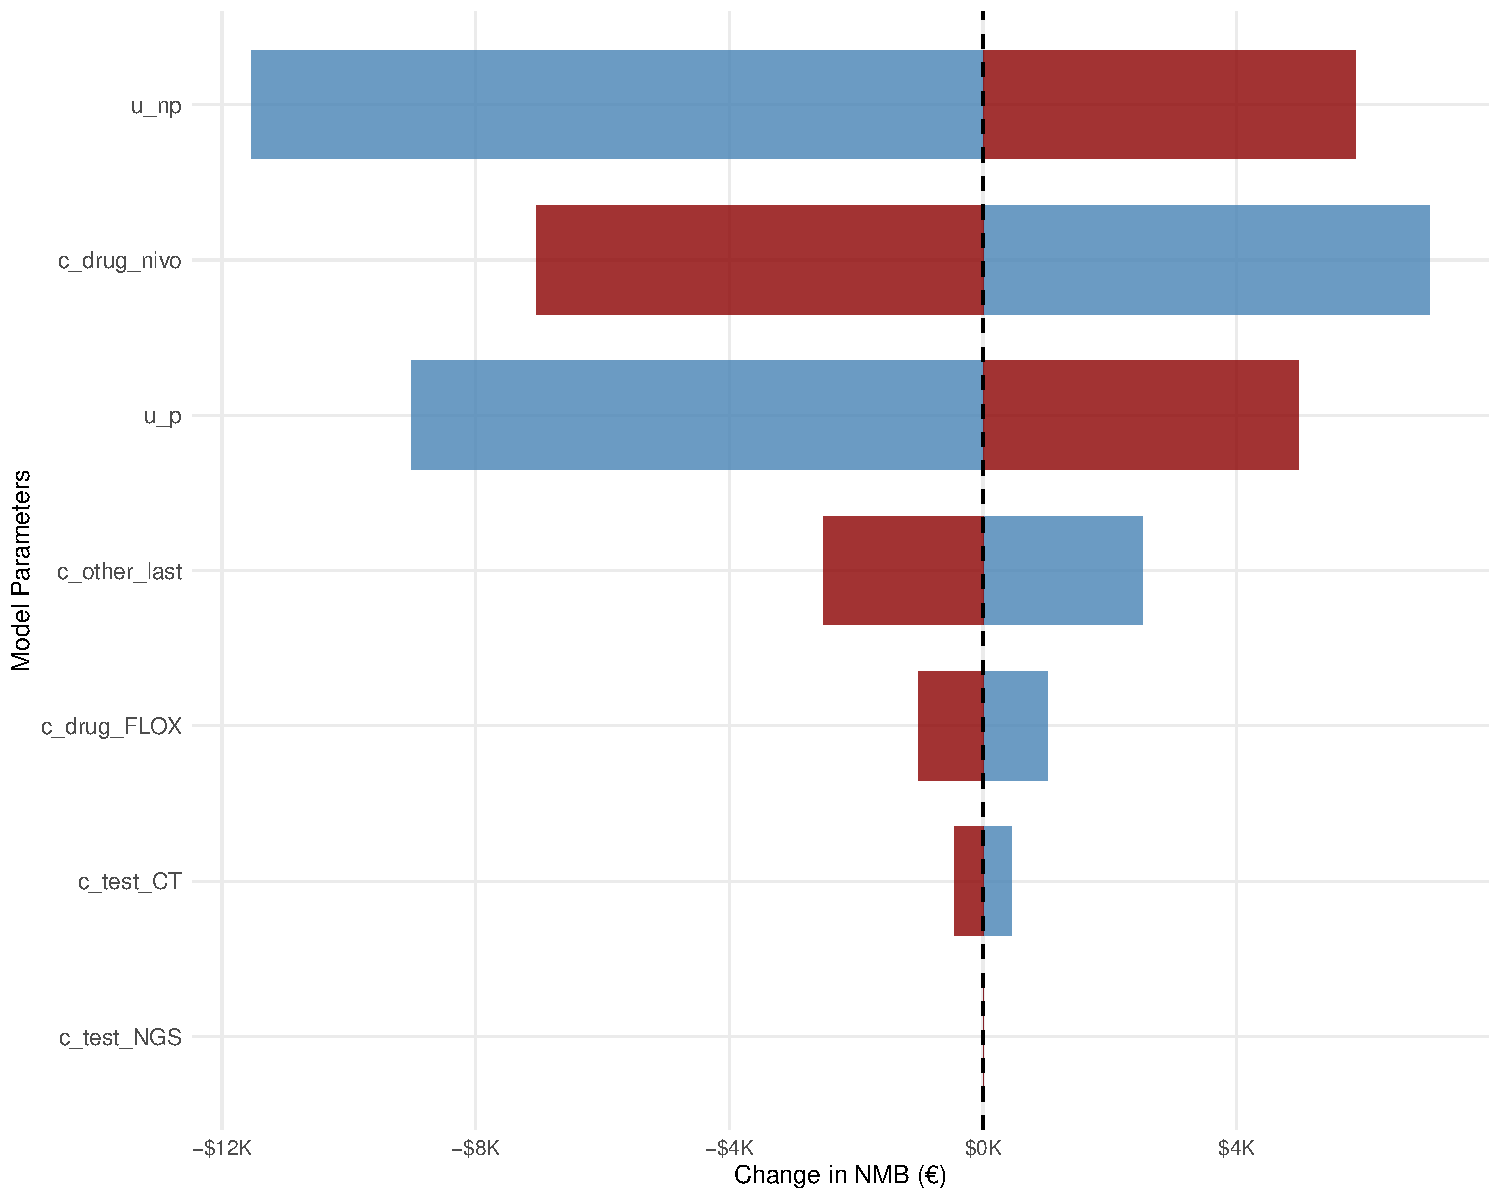
\includegraphics[keepaspectratio]{CEA_files/figure-pdf/tornado-crp-1.pdf}}

}

\caption{Tornado Diagram - CRP-guided Strategy One-Way Sensitivity
Analysis}

\end{figure}%

\begin{figure}[H]

{\centering \pandocbounded{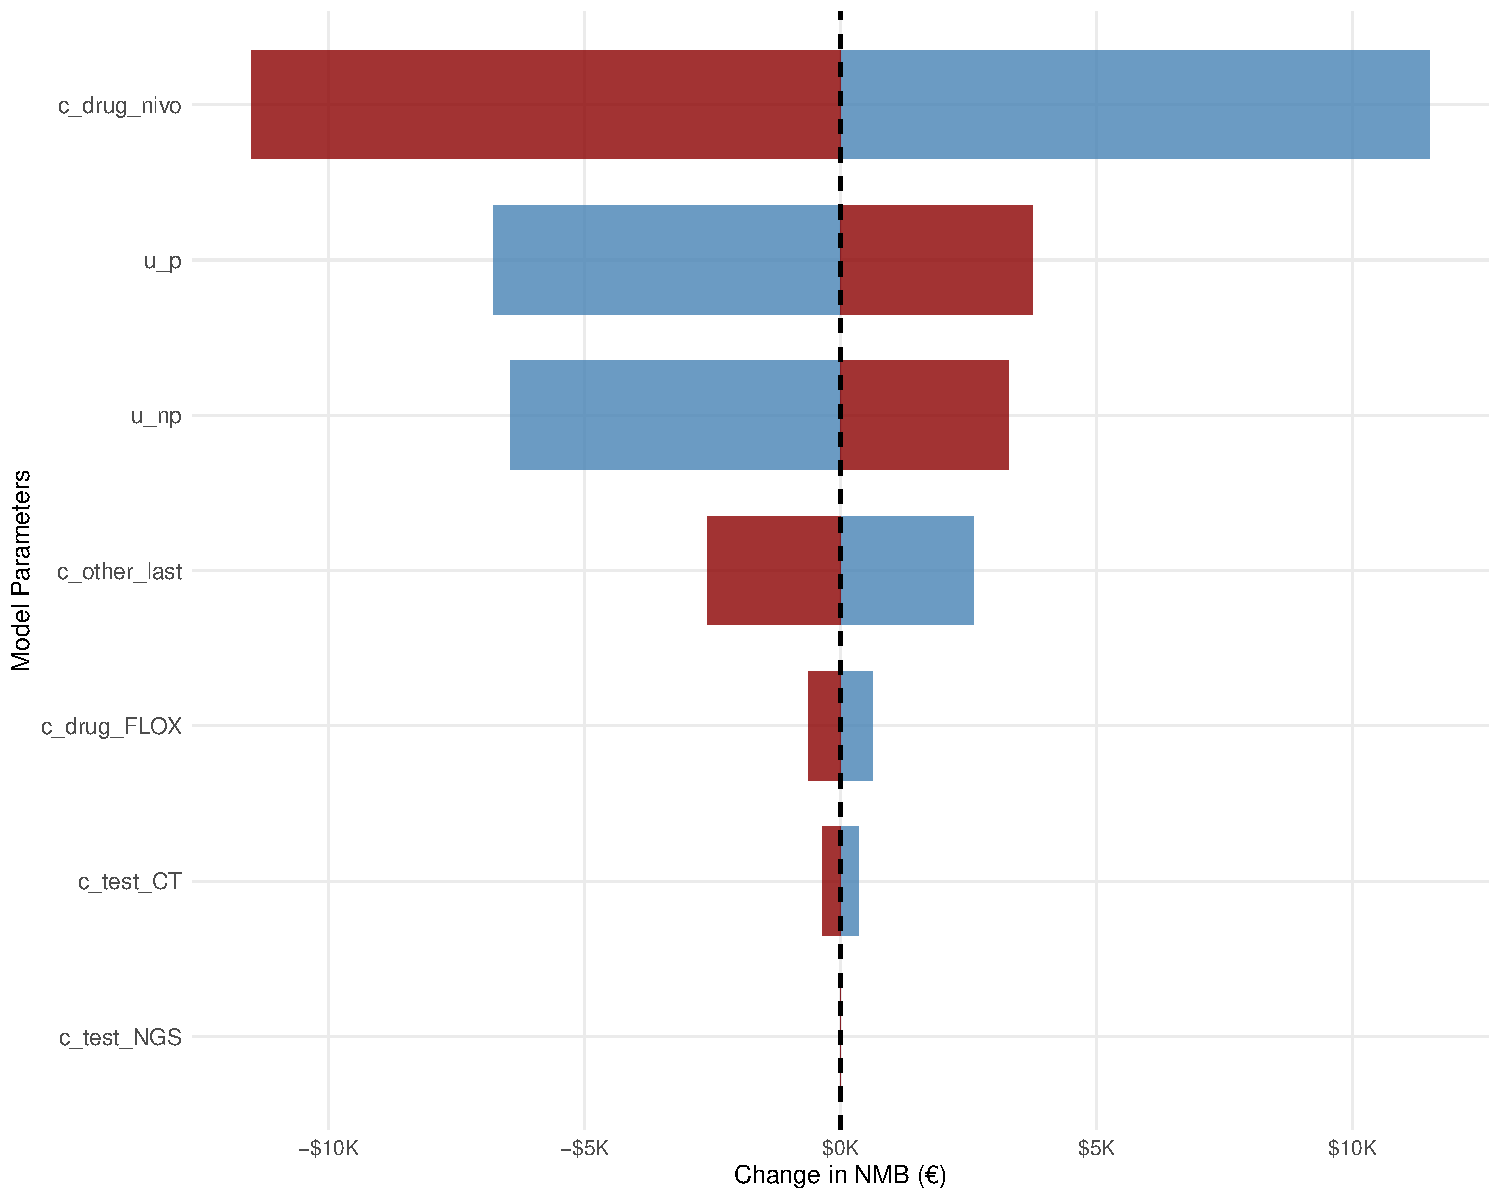
\includegraphics[keepaspectratio]{CEA_files/figure-pdf/tornado-tlr-1.pdf}}

}

\caption{Tornado Diagram - TLR-guided Strategy One-Way Sensitivity
Analysis}

\end{figure}%

\begin{figure}[H]

{\centering \pandocbounded{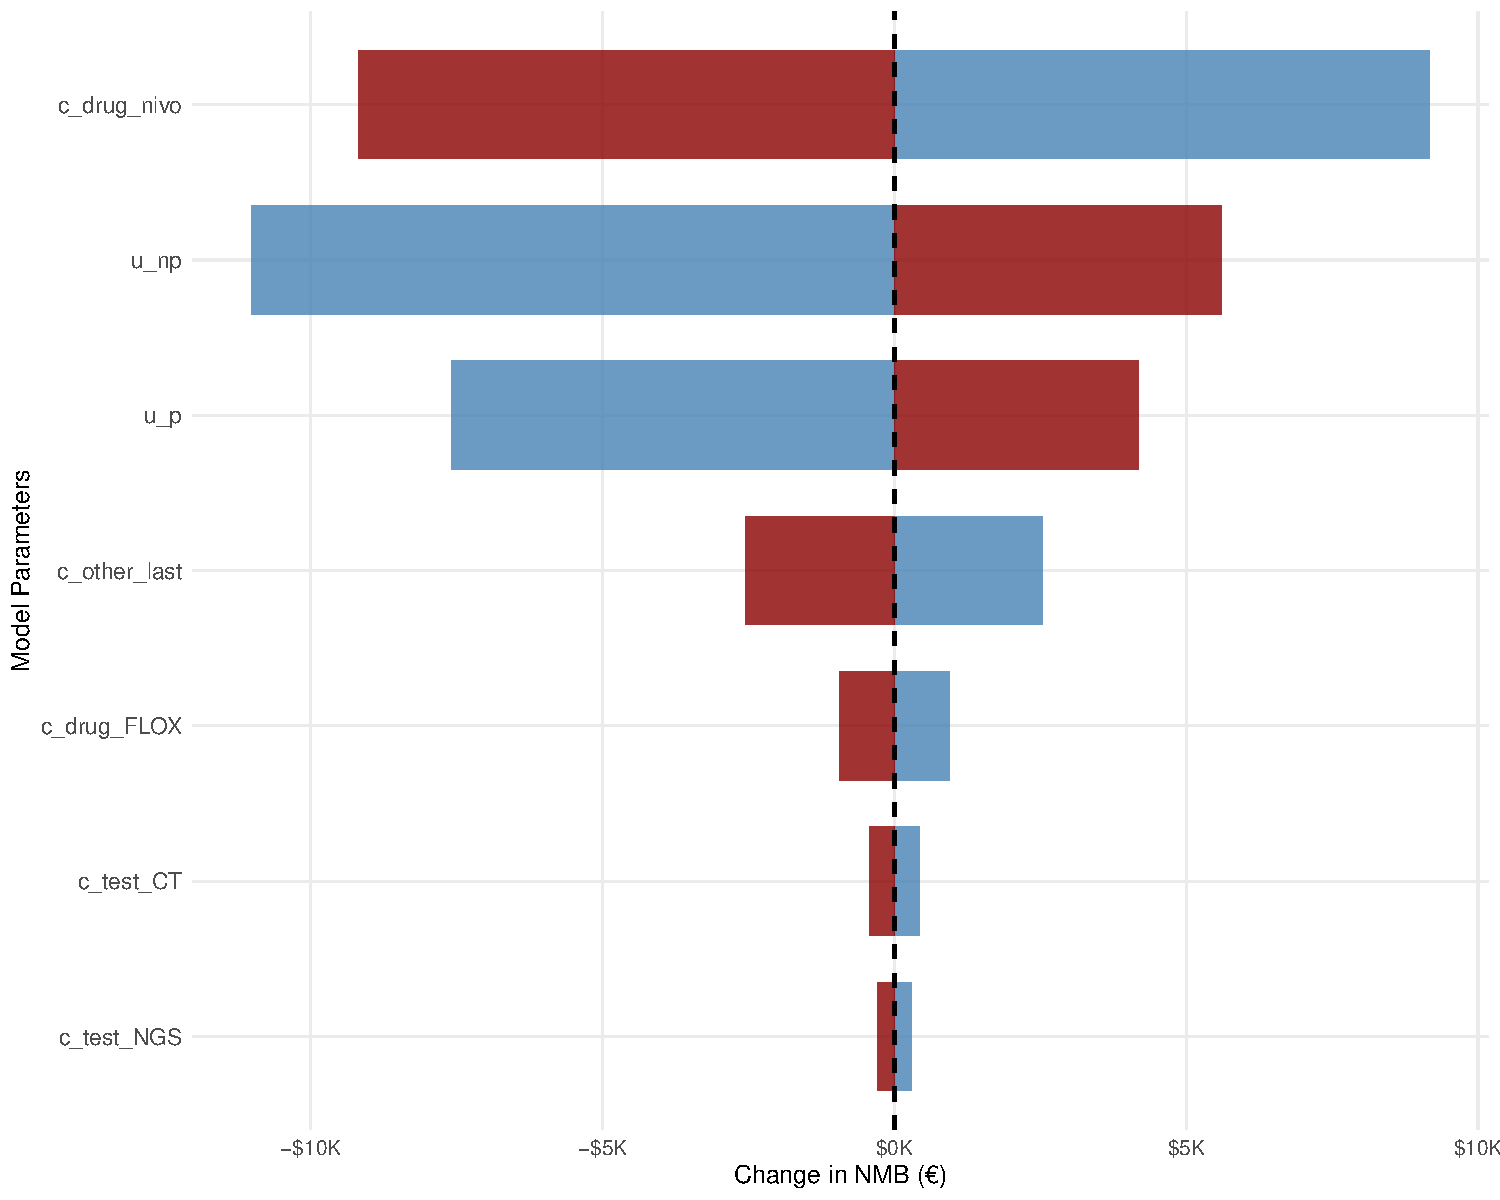
\includegraphics[keepaspectratio]{CEA_files/figure-pdf/tornado-tmb-braf-1.pdf}}

}

\caption{Tornado Diagram - TMB/BRAF-guided Strategy One-Way Sensitivity
Analysis}

\end{figure}%

\newpage

\begin{table}[H]
\caption{Parameter Impact Summary - Most Influential Parameters by Strategy}\tabularnewline

\centering\begingroup\fontsize{10}{12}\selectfont

\begin{tabular}{>{\centering\arraybackslash}p{1.5cm}>{\raggedright\arraybackslash}p{5cm}>{\raggedleft\arraybackslash}p{2.5cm}}
\toprule
Rank & Parameter & Impact on NMB (€)\\
\midrule
\addlinespace[0.3em]
\multicolumn{3}{l}{\cellcolor[HTML]{4472C4}{\textcolor{white}{\textbf{Standard Care}}}}\\
\hspace{1em}1 & Utility (No Progression) & \$15,131\\
\hspace{1em}2 & Utility (Progression) & \$14,392\\
\hspace{1em}3 & End-of-Life Care Cost & \$5,068\\
\addlinespace[0.3em]
\multicolumn{3}{l}{\cellcolor[HTML]{70AD47}{\textcolor{white}{\textbf{CRP-guided}}}}\\
\hspace{1em}1 & Utility (No Progression) & \$17,401\\
\hspace{1em}2 & Nivolumab Cost & \$14,084\\
\hspace{1em}3 & Utility (Progression) & \$13,987\\
\addlinespace[0.3em]
\multicolumn{3}{l}{\cellcolor[HTML]{FFC000}{\textcolor{white}{\textbf{TLR-guided}}}}\\
\hspace{1em}1 & Nivolumab Cost & \$23,444\\
\hspace{1em}2 & Utility (Progression) & \$11,127\\
\hspace{1em}3 & Utility (No Progression) & \$10,105\\
\addlinespace[0.3em]
\multicolumn{3}{l}{\cellcolor[HTML]{C55A11}{\textcolor{white}{\textbf{TMB/BRAF-guided}}}}\\
\hspace{1em}1 & Nivolumab Cost & \$18,559\\
\hspace{1em}2 & Utility (No Progression) & \$17,584\\
\hspace{1em}3 & Utility (Progression) & \$12,692\\
\bottomrule
\end{tabular}
\endgroup{}
\end{table}

\newpage

\section{Probabilistic Sensitivity
Analysis}\label{probabilistic-sensitivity-analysis}

\begin{figure}[H]

{\centering \pandocbounded{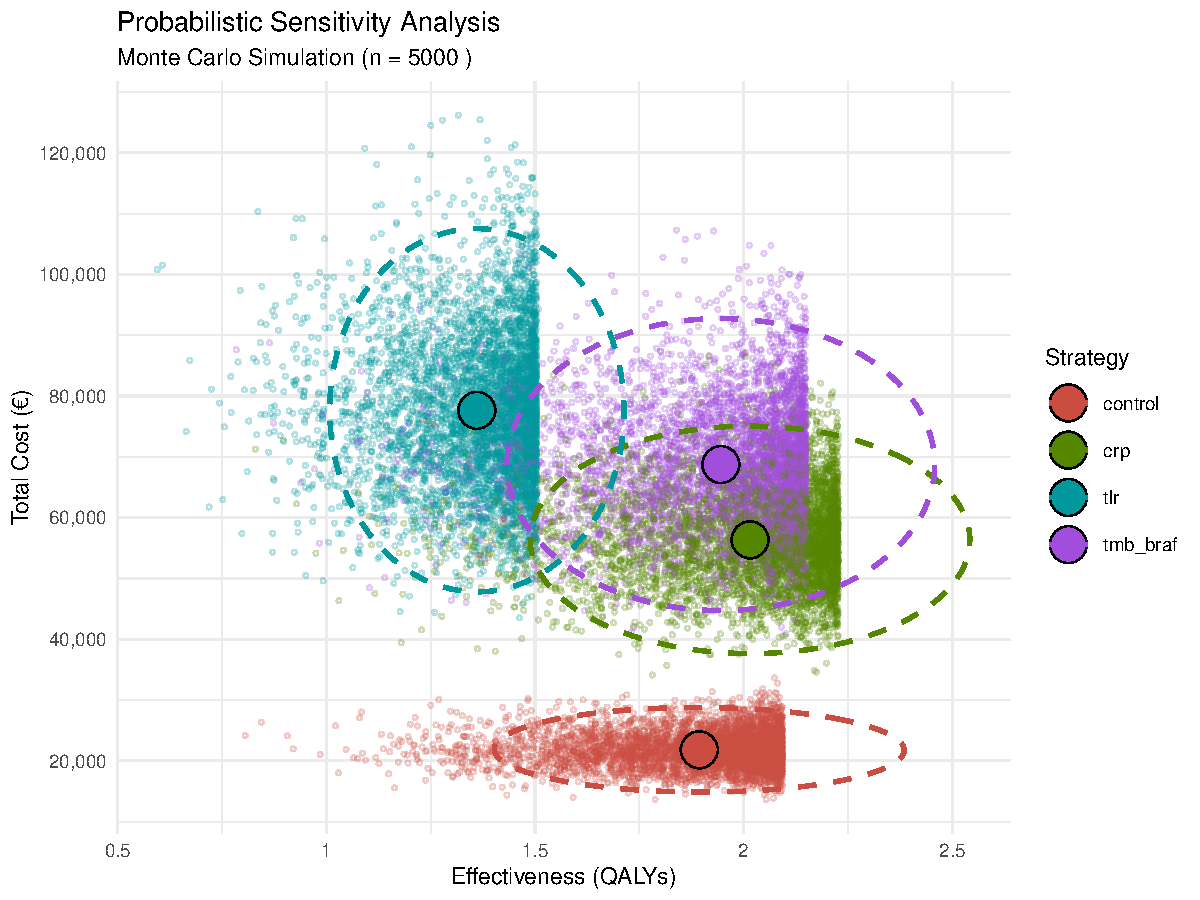
\includegraphics[keepaspectratio]{CEA_files/figure-pdf/psa-scatterplot-1.pdf}}

}

\caption{Cost-effectiveness Scatterplot}

\end{figure}%

\begin{figure}[H]

{\centering \pandocbounded{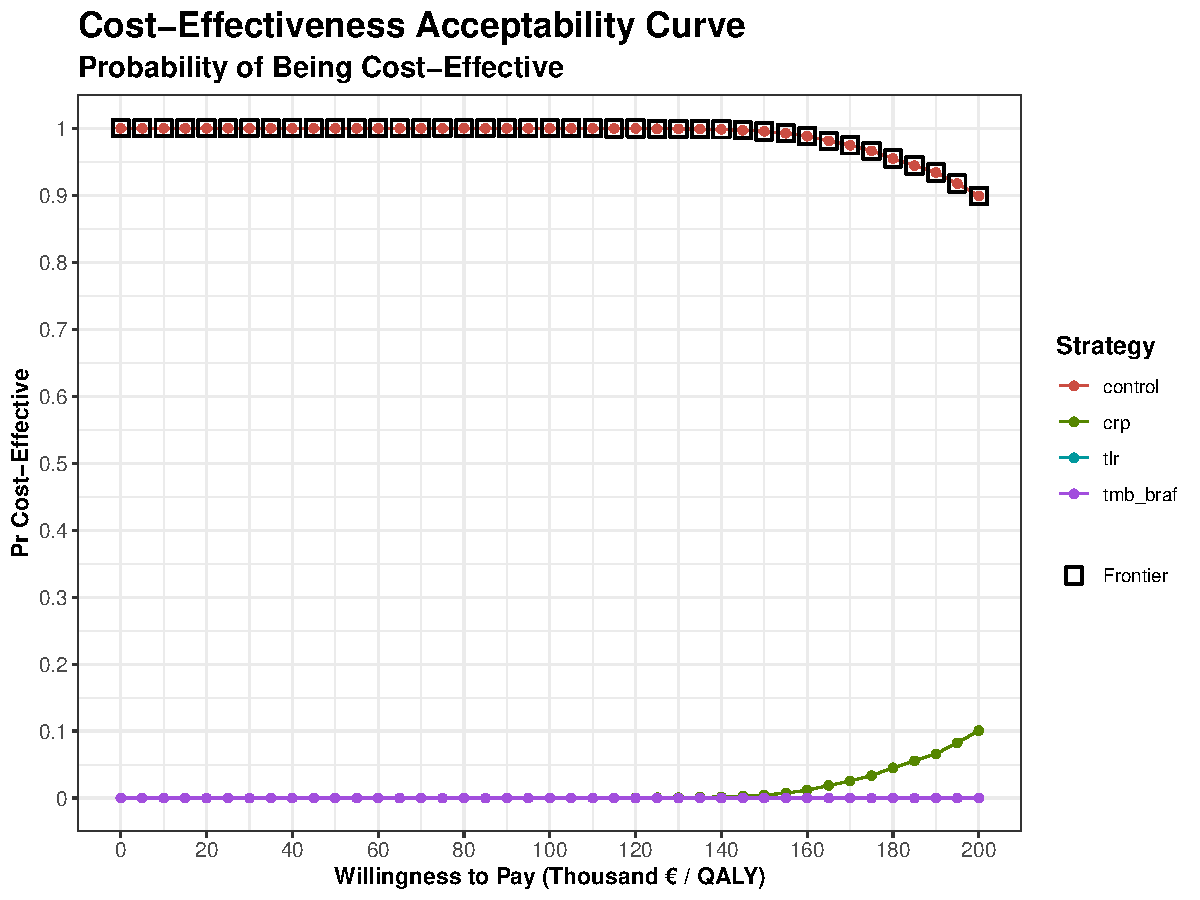
\includegraphics[keepaspectratio]{CEA_files/figure-pdf/ceac-curve-1.pdf}}

}

\caption{Cost-Effectiveness Acceptability Curve}

\end{figure}%

\section{Other Reports}\label{other-reports}

I am working on the following other reports:

\begin{itemize}
\item
  \textbf{Input Parameters Report}: Comprehensive documentation of all
  model input parameters including clinical effectiveness data, cost
  parameters, and utility values with their respective sources and
  uncertainty distributions.
\item
  \textbf{Parametric Survival Analysis Report}: Detailed documentation
  of the parametric survival modeling process, including goodness-of-fit
  statistics for all tested distributions, model selection criteria, and
  validation of the chosen survival models for both overall survival and
  progression-free survival endpoints.
\item
  \textbf{One-Way Sensitivity Analysis (OWSA) Report}: Extended
  sensitivity analysis providing detailed examination of each individual
  parameter's impact on model outcomes, including threshold analyses and
  parameter sensitivity rankings across all strategies.
\end{itemize}

\begin{center}\rule{0.5\linewidth}{0.5pt}\end{center}

\textbf{Report completed on:} 2025-10-07\\
\textbf{Repository:} ben-geisler/METIMMOX-1\\
\textbf{Report version:} 1.0




\end{document}
